%!TEX root = ../3dbook.tex

\setchapterpreamble[u]{\margintoc}

\graphicspath{{LoD2recon/}}
% \renewcommand*{\thelesson}{2.2}

\chapter{3D building reconstruction}%
\label{chap:LoD2recon}

%\newpage
In the previous chapter we discussed how to model 3D objects using the boundary representation.
You learned about data structures to represent the geometry and topology of a 3D object's surface in a very structured and organised way.
In this chapter we will look at how you could create such a structured representation from a much less structured form of 3D geoinformation, namely a point cloud.

In automatic building reconstruction we aim to construct 3D mesh models for individual buildings from some form of elevation measurements, \ie\ a raster-based DSM or a point cloud, without any manual interventions (see Figure~\ref{fig:bk-building-recon}).
\begin{marginfigure}
	\centering
	\begin{subfigure}{\linewidth}
		\includegraphics[width=\linewidth]{figs/bk-pointcloud.png}
		\caption{}%
		\label{subfig:bk-pc}
	\end{subfigure}
\\
	\begin{subfigure}{\linewidth}
		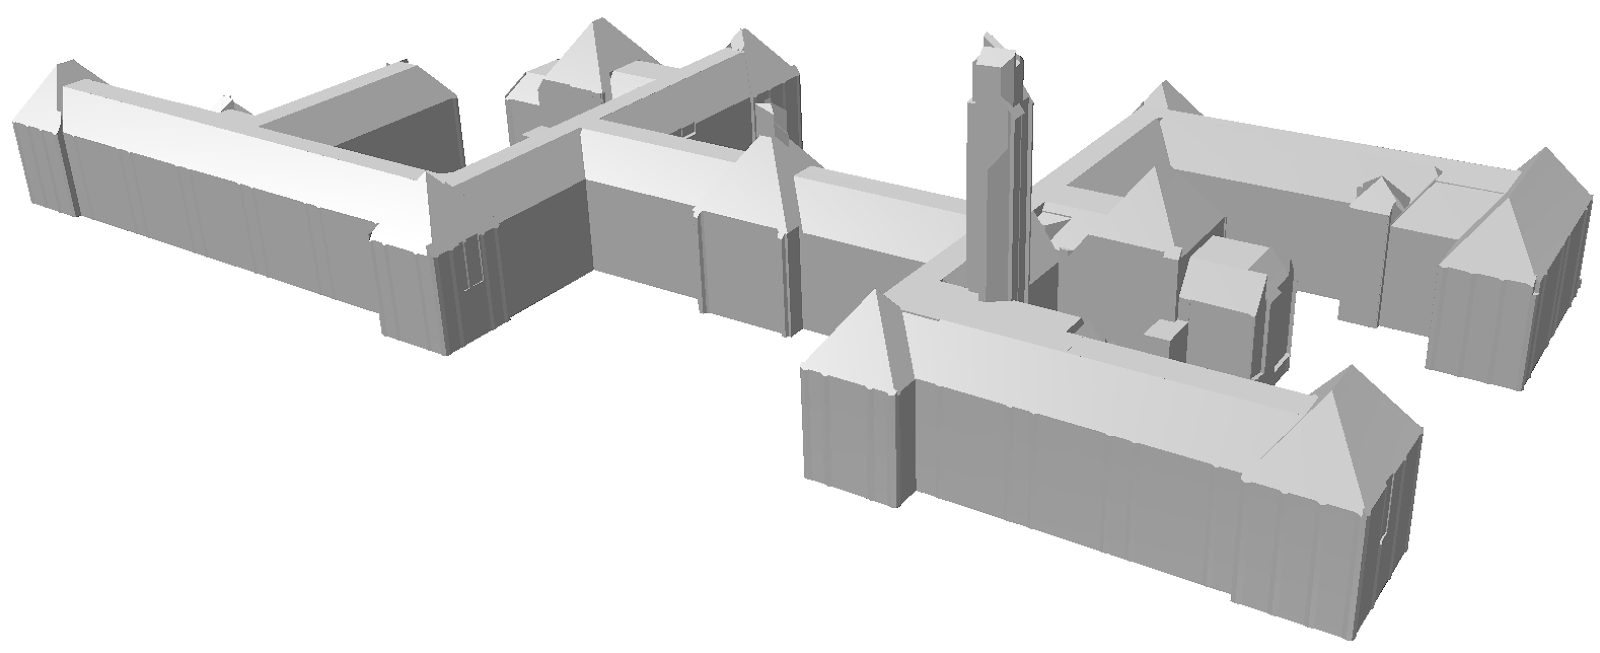
\includegraphics[width=\linewidth]{figs/bk-mesh.png}
		\caption{}%
		\label{subfig:bk-mesh}
	\end{subfigure}
	\caption{Building reconstruction transforms a point cloud (a) into a mesh model (b).}%
	\label{fig:bk-building-recon}
\end{marginfigure}
It can be considered as one step in the geoinformation chain, since we essentially transform 'raw' and unorganised point measurements into more structured and semantically rich 3D models.
Compared to a point cloud, such models are much more useful for applications such as environmental simulations of wind, air pollution, and noise propagation, but also building energy demand estimation and urban planning in general.
Many of these applications require knowledge about the volume or surface area of a building, or the distinction between the interior and exterior of a building, which is evidently much easier to derive from a mesh with a clearly defined boundary than from a point cloud.
In addition, meshes are typically more compact which makes them more efficient to store and process.

This is not to say that meshes are always superior to point clouds. 
For example some of the finer details that may be present in a point cloud could be lost in the mesh representation. 
Furthermore, there is always the risk of introducing new errors and deviations from the original measurement in the building reconstruction process. 
But ultimately, the many benefits of representing a building as a mesh outweigh these disadvantages for many applications.

In this chapter we will first list common challenges and requirements for the building models that are to be constructed. Second, we will look at the important engineering choices in designing a building reconstruction algorithm. And finally, we will discuss one particular approach that was designed to work on Dutch open data in more detail.

%%%
%
\section{Building model requirements and reconstruction challenges}
When designing a building reconstruction method, it is important to carefully consider both the \emph{model requirements} and the \emph{reconstruction challenges}. 
The model requirements specify in detail what properties a reconstructed building model should have. 
Model requirements are mostly application dependent.
For example, an application that performs heavy geometric processing on the building models has stricter geometry and topology requirements than an application that merely visualises the building models.
Reconstruction challenges, on the other hand, are mostly input dependent. 
It is about the characteristics of the input data and the typical shape of the buildings that are present in the input data.
It is relatively easy to design a reconstruction approach for a very high quality point cloud that contains only very simple building shapes, whereas reconstructing complex building shapes from a very sparse and low quality input point cloud is substantially more difficult.

\subsection{Building model requirements}
Following are commonly encountered building model requirements. Notice that the exact requirements will depend on the application.
%An ideal reconstruction method would satisfy all these requirement, but note that in practice we often encounter models that fail in one or several of these.

\begin{description}
	\item[Low complexity] Means that the building model ought to have as few vertices, edges, and faces as possible. Building models with a low complexity are faster to process and take up less storage space.
	\item[High accuracy] The surfaces of the building model should have the lowest possible error with respect to the input point cloud. This error can be measured as the root mean square of all the distances from each input point to the model surface. 
	\item[Geometrically valid] This means among other things that the mesh is 2-manifold, has consistent faces orientation, no duplicated vertices, and no self intersecting geometries. This makes the model generally easier to process since many assumptions can be made about the structure of the mesh. Section~\ref{sec:isovalidity} discusses this (and the relevant ISO19107 standard) in more detail.
	\item[Level of Detail (LoD)] Specifies the degree of generalisation in the roof structure of the reconstructed building model when compared to how the actual building is built. An LoD1 model for example only allows horizontal flat roof surfaces (even if the actual building roof looks different), whereas an LoD2 model also allows for more detailed multi-pitched roof shapes. For the remainder of this chapter we will focus on the more detailed LoD2 models. Section~\ref{sec:lods} discusses the possible LoDs for building models in more detail.
\end{description}

\subsection{Reconstruction challenges}
Why can it be hard to satisfy the model requirements? This depends on the reconstruction challenges. We distinguish between two main categories.

Firstly, there are variations in architectural style. Urban environments can be complex and organised with a high degree of randomness due to their anarchical creation over time. This makes it difficult to design a reconstruction algorithm that is able to model 100\% of the buildings on earth. It is probable that there are always a few cases that violate some of the assumptions made in the building reconstruction method. For example, to simplify a reconstruction approach, it may seem reasonable to assume that buildings are not built on top of each other without touching each other. And while this assumption is valid in more than 99\% of the cases, in practice there are some violations of this assumption (see Figure~\ref{fig:debrug}).
\begin{figure}
	\centering
	\includegraphics[width=\linewidth]{figs/de_brug.jpg}
	\caption{A complex urban environment.}%
	\label{fig:debrug}
\end{figure}
	
Secondly, we need to consider the quality and completeness of the input data. This mostly relates to how the input data, \ie\ the point cloud, was acquired (compare \eg\ Figure~\ref{fig:pc-quality:low} to \ref{fig:pc-quality:high}).
\begin{marginfigure}
	\centering
	\begin{subfigure}{\linewidth}
		\includegraphics[width=\linewidth]{figs/rdam16_ahn2.png}
		\caption{}%
		\label{fig:pc-quality:low}
	\end{subfigure}
	\\
	\begin{subfigure}{\linewidth}
		\includegraphics[width=\linewidth]{figs/rdam16_d.png}
		\caption{}%
		\label{fig:pc-quality:high}
	\end{subfigure}
	\caption{Varying point cloud qualities. a) low point density with missing facades, b) high point density and points on facades.}%
	\label{fig:pc-quality}
\end{marginfigure}
Most building reconstruction methods work with point clouds that are captured from an airplane. 
This is the most efficient way to cover large areas, but it also means that not all the exterior surfaces of a building are captured due to occlusion. In particular facades and the underside of overhanging structures may be missing in such datasets. 
If a surface is missing in the point cloud we need to compensate for that with assumptions on what we expect the building to look like. 
For instance, we could assume that facades are always vertical so that we can simply model a vertical plane from the roofline to the ground. 
However, while this is reasonable for the majority of buildings there are bound to be some exceptions.
Other point cloud properties are also important. For example the point density is indicative for the smallest details that we can reliably detect in the point cloud. Consequently we can not reasonably expect to see smaller details in the reconstructed building model unless very strong assumptions are taken on the type of building shape that is modelled. Some surface materials can also lead to problems. Glass surfaces for example are notoriously difficult to measure with airborne acquisition techniques, leading \eg\ to holes in the roof surface which can lead to problems in a building reconstruction method.


%%%
%
\section{Data driven versus model driven building reconstruction}
Building reconstruction has been a popular topic among researcher over the last few decades. 
Many approaches exist that vary in the expected type and resolution or density of input data, the precise model requirements, and in how restricted they are to a particular architectural style.
One could classify these methods on a linear scale with on one extreme the purely so-called \emph{data  driven} approaches and on the other extreme the purely so-called \emph{model driven} approaches.

\begin{marginfigure}
	\includegraphics[width=\linewidth]{figs/data-driven.png}
	\caption{Data driven reconstruction based on a triangulation of the input points \citep{Axelsson99}}%
	\label{subfig:data-driven}
\end{marginfigure}
The data driven approach strongly relies on the quality and completeness of the input data.
The resulting building models have a good data fit, but a high complexity (high number of faces).
Defects in the input data are likely to cause problems in the building model, such as holes and non-2-manifoldness.
Examples of the data driven approach are methods that triangulate directly the input point cloud (see Figure~\ref{subfig:data-driven}).

\begin{marginfigure}
	\includegraphics[width=\linewidth]{figs/model-driven.png}
	\caption{Model driven reconstruction by fitting parametrised roof models \citep{Lafarge10}}%
	\label{subfig:model-driven}
\end{marginfigure}
The model driven approach, on the other hand, relies on strong modelling assumptions about the building shape.
This typically results in models with a low complexity, but a poorer fit with the input points when compared to a purely data driven approach.
Because the model driven approach does not rely so heavily on the quality of the input, defects in the input point cloud are less likely to lead to problems in the building model.
Examples of the model driven approach are methods that fit pre-defined roof shapes such as a simple gable roof to a point cloud (see Figure~\ref{subfig:data-driven}). 
Such a method will only work for buildings for which a pre-defined roof shape is available.
Yet, if this the case it can already work reliably for a very sparse point cloud.

Clearly both approaches have limitations. The most advanced building reconstruction methods, including the one discussed below, try to combine the best of both to come to an optimal compromise, \eg\ a method that has both a good datafit and a high degree of flexibility in building shapes but also a low complexity and perfect geometric validity. However, be aware that such a mixed approach combines not only the advantages, but likely also the disadvantages of both approaches to some degree.

% Table~\ref{tab:data-vs-model-driven} gives an overview of the various trade-offs between the data driven and the model driven approach. 
% \begin{table}[]
% 	\centering
% 	\begin{tabular}{p{7cm}|p{7cm}}
% 	Data driven & Model driven \\
% 	\hline
% 	Requires high quality input	& Suitable for low quality input \\
% 	Good data fit	& Possibly loose data fit \\
% 	Sensitive to defects in input data &  Can overcome input defects to some extent \\
% 	High model complexity & Low model complexity \\
% 	No assumptions on building shape	&  Strong assumptions on building shape\\
% 	Can deal with large variety of building shapes	& Limited to specific building shapes\\
% 	No semantics (\ie\ no distinction roof, wall and floor faces) & Has semantics
% 	\end{tabular}
% 	\caption{Trade-offs in data driven versus model driven reconstruction}%
% 	\label{tab:data-vs-model-driven}
% \end{table}
% Notice that this table describes merely the two extremes, and that mixed approaches also exist.
%The important thing is that you learn to understand about the 


%In conclusion, it should be clear that there is no such thing as a perfect . 

% model only superstructures with model-driven approach (iconisation)


\section{Automatic LoD2 reconstruction for the Netherlands}
% design context
In this section we will discuss an automatic LoD2 reconstruction method that I developed to work with Dutch open data\marginnote{the AHN3 point cloud and the BAG building footprints}. 
The output of this method should have both a good data fit and a low model complexity and is aimed to have completely valid geometry output. 
This means the resulting models are suitable for various kinds of environmental simulation applications.

% modelling assumptions
\subsection{Modelling assumptions}
The following assumptions are taken in the reconstruction method. They are deemed reasonable for the Dutch input datasets that the method was designed on, and with these assumption the reconstruction problem is somewhat simplified.

\begin{description}
	\item[piecewise planar] The shape of a building can be adequately approximated using planar faces that are detectable from the point cloud.
	\item[2.5D with vertical walls] The roof of the building is 2.5D and all walls are vertical. This implies the 3D building model can be extruded from a 2D planar partition of the roof. The 2.5D assumption is quite reasonable for airborne point cloud, because each building is only scanned from above anyhow.
	\item[classified point cloud] A reliable classification of the input point cloud is expected, \ie\ at least a building and a terrain (ground) class must be present. This is the case for the AHN3 dataset that is used.
	\item[footprints are available] Apart from a point cloud the method also takes 2D building footprints as input. These are used to crop the point cloud for each building. It is assumed that the footprints are up-to-date and well aligned with the point cloud.
\end{description}

% data or model driven?
The method can be classified as a mix between the purely data and model driven approaches as discussed in the previous section. 
Consequently it also mixes the benefits and trade-offs of both extremes.
For example, instead of forcing complete roof shapes on a point cloud, it is only assumed a building is composed of planar surfaces.
This makes the method more flexible compared to a purely model driven approach that fits a pre-defined roof shape, since it should be able to handle any possible roof shape that can reasonably be approximated with (large) planar surfaces while still mainting a low model complexity.
However, if a plane cannot be fitted to a part of the roof due to defects in the point cloud, that part may lead to errors in the resulting building model.


% overview method
\subsection{Method overview}
Figure~\ref{fig:method-overview} illustrates the six main steps of the algorithm. The main idea is to compute a so-called \emph{roof-partition}; a planar partition of the footprint where each face corresponds to a planar piece of the roof and is labeled with a roof plane. Prior to creating the roof-partition the roofplane and line features must be extracted from the point cloud (Figure~\ref{fig:method-overview} step 2 and 3). And once the roof-partition is available, the 3D building model can be generated through extrusion (Figure~\ref{fig:method-overview} step 6).
\begin{figure}
	\centering
	\includegraphics[width=\linewidth]{figs/reconstruction-overview.pdf}
	\caption{The main steps in the reconstruction algorithm. 1) the classified (aerial) point cloud is cropped on the 2D footprint, 2) planes and their boundaries are detected in the point cloud, 3) from the roof planes the intersection lines and boundary lines are extracted, 4) the lines are regularised and projected onto the 2D footprint, 5) the roof-partitions is created. This is a DCEL where each face is labeled with the corresponding plane (from 2, compare colors). 6) the roof-partition is extruded into a 3D mesh. \\If a terrain plane is assigned to a face from the roof-partition, that face is removed (2 and 5).}%
	\label{fig:method-overview}
\end{figure}

%The method consists of five steps.
%\begin{enumerate}
%	\item Plane detections
%	\item Line detection and regularisation
%	\item Subdivision of the footprint
%	\item Graph-cut optimisation
%	\item Extrusion
%\end{enumerate}

\subsubsection{Feature extraction}
% \begin{kaobox}[frametitle=\faExternalLink\ To read or to watch.]
% 		The reader is advised to read the section on shape detection in the Chapter \emph{Point cloud processing} in the book \href{https://github.com/tudelft3d/terrainbook/releases}{\emph{Computational modelling of terrains}}.
% \end{kaobox}
The roof-partition is made using lines that are derived from roof planes that are extracted from the building point cloud.
The roof planes are detected using a region-growing algorithm and then two type of lines are derived from the planes: boundary lines and intersection lines (see Figure~\ref{fig:method-overview} step 3).
The boundary lines are created by detecting lines in the boundary of the $\alpha$-shape of each detected roof plane.
The intersection lines are created where adjacent planes intersect, such as on the top of a gable roof.

Before the boundary and intersection lines are used to partition the footprint, they are regularised.
The goal of line regularisation is to remove duplicate lines and thereby reduce the complexity of the roof-partition.
For example, the line on top of the gable roof in Figure~\ref{fig:method-overview} is detected three times: once as an intersection line and twice as a boundary line (once for each incident roof plane).
After line regularisation only a single line remains.
After projecting the detected lines to 2D, line regularisation is done in two steps: orientation clustering and distance clustering (see Figure~\ref{fig:lineclust}).

Orientation clustering is performed first, and in this step lines that have approximately the same orientation in the 2D plane are put in the same cluster. For example in Figure~\ref{fig:lineclust:2}, there are two dominant orientations that each form a cluster of lines. Withing each orientation cluster the angle between the lines is relatively small, whereas the angle between lines in different clusters is large.
\begin{figure}
	\centering
	\begin{subfigure}[b]{0.48\linewidth}
		\includegraphics[angle=90,width=\linewidth]{figs/line-clustering/slice1.pdf}
		\caption{Detected lines}%
		\label{fig:lineclust:1}
	\end{subfigure}
	\quad
 	\begin{subfigure}[b]{0.48\linewidth}
		\includegraphics[angle=90,width=\linewidth]{figs/line-clustering/slice2.pdf}
		\caption{Orientation clustering}%
		\label{fig:lineclust:2}
	\end{subfigure}
\\
	\begin{subfigure}[b]{0.48\linewidth}
		\includegraphics[angle=90,width=\linewidth]{figs/line-clustering/slice3.pdf}
		\caption{Distance clustering}%
		\label{fig:lineclust:3}
	\end{subfigure}
\quad
	\begin{subfigure}[b]{0.48\linewidth}
		\includegraphics[angle=90,width=\linewidth]{figs/line-clustering/slice4.pdf}
		\caption{Regularised lines}%
		\label{fig:lineclust:4}
	\end{subfigure}	
	\caption{Line regularisation through clustering. }%
	\label{fig:lineclust}
\end{figure}

Next, distance clustering is performed.
This divides each orientation cluster into one or more distance clusters.
This is done by computing for each orientation cluster the distances between the lines it contains.
Groups of lines with a small distance with respect to each other are put in their own distance cluster, weheras the distance between different distance clusters is large (see Figure~\ref{fig:lineclust:3}).

Finally, one average line is computed for each distance cluster (Figure~\ref{fig:lineclust:4}).

\subsubsection{Construction of the roof-partition}
After the lines are detected and regularised they are used to subdivide the footprint into a planar partition called the roof-partition.
A doubly connected edge list (DCEL) is used to represents the full topology of the planar partition of the footprint, that is referred to as the \emph{initial roof-partition}.
This means that each intersection is explicitly represented with a vertex.
In addition there are no dangling edges.
The use of a DCEL allows for easy traversal and manipulation of the roof-partition, \eg\ for the extrusion to a 3D mesh in the last step.


Depending on the number of lines that remain after regularisation, the initial roof-partition may still have a high complexity; it may contain many small faces.
To further reduce the complexity of the roof-partition and to simultaniously assign an optimal roofplane to each face, an optimisation step is performed\marginnote{Graph-cut optimisation is used. The details on how graph-cut optimisation works are outside the scope of this course.}.
In this step a roof plane is assigned to each face in the roof-partition (see Figure~\ref{fig:method-overview} step 5).
This is done in such a way that 1) the total error with the input point cloud is minimised and 2) the total length of the edges between faces of a different roof plane is minimised.
This  optimisation thus seeks an optimal balance between respectively a good data fit and a low complexity of the roof-partition.
After the optimisation is complete, the edges for which the two incident faces are assigned to the same roof plane are removed from the partition.
The faces in the resulting \emph{final roof-partition} are referred to as \emph{roof-parts}.

\subsubsection{Extrusion}
\label{sec:extrusion}
The final roof-partition is transformed into a 3D building mesh using extrusion.
This is done by exploiting the topological information that is available in the the DCEL of the roof-partition, as illustrated in Figure~\ref{fig:extrusion}.
\begin{figure}
	\centering
	\begin{subfigure}[b]{0.45\linewidth}
		\includegraphics[width=\linewidth]{figs/2DDCEL.pdf}
		\caption{}%
		\label{subfig:2ddcel}
	\end{subfigure}
	\quad
	\begin{subfigure}[b]{0.45\linewidth}
		\includegraphics[width=\linewidth]{figs/3DDCEL.pdf}
		\caption{}%
		\label{subfig:3ddcel}
	\end{subfigure}
	\caption{The roof-partition is represented as a DCEL (a). When extruding to a 3D mesh (b), each edge in the roof-partition becomes a wall face in the 3D Mesh. Each vertex in the roof-partition (\eg\ $v_1$) needs to be replicated for each incident face: \eg\ $v_{1A}$, $v_{1B}$, $v_{1C}$ in the 3D Mesh.}%
	\label{fig:extrusion}
\end{figure}
Notice that the building mesh consists of three types of faces, \ie\ the floor, the roof and the wall faces.
These are generated from the roof-partition in separate procedures.

\begin{marginfigure}
	\centering
	\includegraphics[width=\linewidth]{figs/extrusion-edge.pdf}
	\caption{The edge $e$ (comprising of two halfedges $e_A$ and $e_B$) is incident to two faces ($f_A$ and $f_B$) and two vertices ($v_1$ and $v_2$). In case of a roof-partition, the height at $v_1$ on face $f_A$ is denoted as $h_{1A}$.}%
	\label{fig:extrusion-notation}
\end{marginfigure}

\begin{description}
\item[floor face] The geometry of the floor face consists of the edges in the roof-partition that are incident to the exterior to the footprint. The elevation of the floor face can either be set to the lowest ground point around the building, or if a terrain mesh is available it can be made exactly fitting with the terrain by computing the intersection with that terrain mesh and setting the vertex elevations accordingly. 

\item[wall faces] These are vertical faces that connect the floor face with the roof faces. They are extruded from the edges in the roof-partition that have one or two incident roof parts. Depending on the plane configuration of the incident roof parts an edge is extruded differently. Figure~\ref{fig:extrusion-cases} shows a few possible cases (there are more).
\begin{figure}
	\includegraphics[width=\linewidth]{figs/extrusion-edge-cases.pdf}
	% \caption{Various possible roof face configurations at edge $e$}%
	\caption{Determining wall face geometry and vertex order. $h_{1A}$ denotes the elevation at vertex $v_1$ on face $f_A$ (see Figure~\ref{fig:extrusion-notation}).}%
	\label{fig:extrusion-cases}
\end{figure}
Notice that an edge in the roof-partition can generate 0 (if the incident planes intersect exactly at the edge), 1 or 2 wall faces.
Also notice that the order of the vertices of a wall face (so that they are oriented counter-clockwise around the face normal that points to the exterior of the mesh) is completely determined by the plane configuration case at the edge.

Special attention needs to be paid to vertices that are extruded to more than two elevations such as $v_1$ in Figure~\ref{subfig:2ddcel}.
To get a topologically correct building mesh, the extruded vertices should become part of all their incident wall faces.
Vertex $v_{1B}$ should thus also be inserted in the boundary ring of the blue face in Figure~\ref{subfig:3ddcel}, despite the fact it is co-linear with $v_{1A}$ and $v_{1C}$.

\item[roof faces]  Each roof part in the interior of the roof-partition will generate a roof face in the building mesh. The planimetric geometry of the roof faces is identical to the faces in the roof-partition. The vertex elevations are found by projecting the 2D vertices to the plane of the roof-part.
\end{description}

%%%
%
\section{Notes and comments}
\citet{Rottensteiner14} gives an overview of building reconstruction methods.

If you want to know more about the graph-cut optimisation method to optimise the roof-partition have a look at the paper from \citet{Zebedin08}.

A good example of a true 3D building reconstruction method (no 2.5D assumption) is the work of \citet{Nan2017}

%%%
%
\section{Exercises}

\begin{enumerate}
  \item Explain the advantages of 2-manifoldness in a building model
  \item Complete the table of possible plane configurations in Figure~\ref{fig:extrusion-cases}.
  \item Could a non-manifold edge be created in the extrusion that is described in Section~\ref{sec:extrusion}? If so, describe how that could happen.
\end{enumerate}
